\documentclass{beamer}
\usepackage{multicol}

\usetheme[progressbar=frametitle]{metropolis}
\setbeamertemplate{frame numbering}[fraction]
\useoutertheme{metropolis}
\useinnertheme{metropolis}
\usefonttheme{metropolis}
\usecolortheme{spruce}
\setbeamercolor{background canvas}{bg=white}

\title[Cut-off Coulomb]{The optical properties of Hydrogen plasma described in the frame of the fully quantum method based on a cut-off Coulomb model potential}
\author{Nenad M.~Sakan$^{1}$*, Zoran J. Simi\'c$^{2}$, and Momchil Dechev$^{3}$}
\institute{\it $^{1}$ Institute of Physics, Belgrade University, Pregrevica 118, 11080 Zemun, Belgrade, Serbia\\
           $^{2}$ Astronomical Observatory, Volgina 7, 11060 Belgrade, Serbia\\
           $^{3}$ Institute of Astronomy and National Astronomical Observatory, Bulgarian Academy of Sciences, 72, Tsarigradsko chaussee Blvd. Sofia, Bulgaria\\
           {\bf nsakan@ipb.ac.rs}}
% \email{\bf nsakan@ipb.ac.rs}

\date{}

\begin{document}

\begin{frame}
 \titlepage
\end{frame}


\begin{frame}{The goal - as much processes as possible}

{\Large Up untill now it is work in progress:}

\begin{itemize}
 \item Transport properties - to be included
 \item Optical properties
 \begin{itemize}
    \item Free-free transitions (inverse Bremsstrahlung) - included
    \item Bond-free transitions (Photoionization) - included
    \item Bond-bond transitions - partially included work in progress
 \end{itemize}
 \item Plasma-emiter interraction - model one
\end{itemize}

{\Large the results are proven to be usable}

\end{frame}

\begin{frame}{QM model potential pt.1}
    Multiparticle system is represented with single particle system that has a modeled interaction with plasma by the means of modeling pseudoptential.
    
    Cut-off Coulomb potential
    
    \begin{equation}
        \label{eq:U0} U_{c}(r) = \left\{
        \begin{array}{c c}
        - \displaystyle \frac{e^2}{r} + \displaystyle \frac{e^2}{r_c},
        \qquad            0 < r \le r_{c},
        \\
        \displaystyle 0 ,              \qquad      r_{c} < r < \infty,
\end{array}
\right.
\end{equation}
    
\end{frame}

\begin{frame}{QM model potential pt.2}
\centering
%    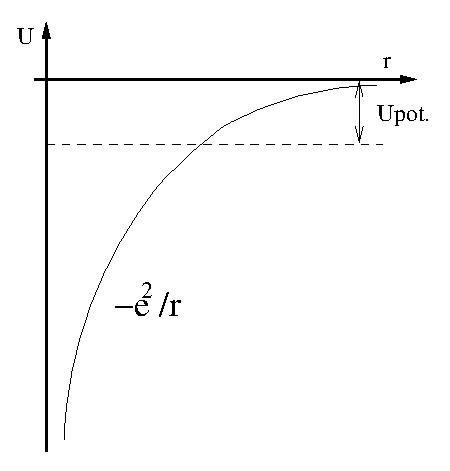
\includegraphics{./fig/prva_slika.eps}
%    \caption{model potential}
        $$
        \label{eq:U0} U_{c}(r) = \left\{
        \begin{array}{c c}
        - \displaystyle \frac{e^2}{r} + \displaystyle \frac{e^2}{r_c},
        \qquad            0 < r \le r_{c},
        \\
        \displaystyle 0 ,              \qquad      r_{c} < r < \infty,
        \end{array}
        \right.
        $$
        
    \begin{itemize}
     \item Close vicinity of the emitter - Coulomb
     \item Far field - average plasma potential
     \item Cut-off plasma-emiter interaction
    \end{itemize}

\end{frame}


\begin{frame}{QM model potential pt.3}
    Behind all quantities in a dipole approach lies a dipole matrix element. For instance for the photoionization the dipole matrix element is given by 
    
    $$
    \hat{D}_{n,l;\;E,l'} = \displaystyle \int P_{nl} r P_{El'} dr.
    $$

    $P$ is analytically and numericaly solvable for used cut-off Coulomb model potential. Cut-off Coulomb potential is a simple approximation, but it is open for inclusion of more complex models of plasam interaction.
\end{frame}

\begin{frame}{Expected area of good agreement}
\begin{figure}
    \includegraphics[scale=0.40,angle=-90]{fig/color_rc.eps}
\hfill    
    \includegraphics[scale=0.40,angle=-90]{fig/color_N.eps}
\end{figure}
Dense plasma: $5 \times 10^{20} \ cm^{-3} \ge N_e \ge 1 \times 10^{18}\ cm^{-3}$
\end{frame}

\begin{frame}{Up untill now pt.1}
    Hydrogen model yeilded good agreement with the theory of unperturbed emmiter, e.g. pure Coulomb model potential, the Inglis–Teller behaviour is confirmed. The results ae usable for modeling
    
    \begin{figure}
        \includegraphics[scale=0.25,angle=-90]{fig/preseci_2_U0.eps}
    \hfill    
        \includegraphics[scale=0.25,angle=-90]{fig/preseci_4_U0.eps}
    \end{figure}

like a displayed cross sections.
\end{frame}

\begin{frame}{Up untill now pt.2}
    Hydrogen model is proven, the cut-off Coulomb potential is used in several calculations up untill now.
    
    \begin{itemize}
     \item Mihajlov, A.A., Sakan, N.M., Sre{\'c}kovi{\'c}, V.A., {Vitel}, Y., ``Modeling of continuous absorption of electromagnetic radiation in dense partially ionized plasmas.'' J. Phys. A 2011, 44,~095502.
     
     \item {Mihajlov}, A.A., {Sre{\'c}kovi{\'c}}, V.A., {Sakan}, N.M., ``Inverse Bremsstrahlung in Astrophysical Plasmas: The Absorption Coefficients and Gaunt Factors.'', J. Astrophys. Astron., 2015, 36,~635--642.
    \end{itemize}
\end{frame}
    
\begin{frame}{Up untill now pt.3}

    \begin{itemize}
     \item {Sre{\'c}kovi{\'c}}, V.A., {Mihajlov}, A.A.,``The application of the cut-off Coulomb potential for the calculation of a continuous spectra of dense hydrogen plasma.'', Mem. S. A. I. Suppl., 2005, 7,~221--224.
     
     \item Sakan, Nenad M. and Srećković, Vladimir A. and Simić, Zoran J. and Dimitrijević, Milan S., ``The Application of the Cut-Off Coulomb Model Potential for the Calculation of Bound-Bound State Transitions'', Atoms, 2018, 6, 1, 4
    \end{itemize}
\end{frame}

\begin{frame}{NOW pt.1}
    The wavefunctions for the bond states are calculated, the convergence towards unperturbated ones are tested
    
    \begin{figure}
        \includegraphics[scale=0.32,angle=-90]{fig/psi_n_3_l_0.eps}
    \hfill    
        \includegraphics[scale=0.32,angle=-90]{fig/psi_n_3_l_1.eps}
    \end{figure}

    The model yielded results for dipole matrix element that converged towards unperturbated, pure Coulomb model ones.
\end{frame}

\begin{frame}{NOW pt.2}
    The code for inclusion a more complex model potentials, e.g. for Ar I is finished and the results are tested
    
    \begin{figure}
        \includegraphics[scale=0.35,angle=-90]{fig/psi_Ar_n_5_l_0.eps}
    \end{figure}

    
    The dipole matrix elemets as well as oscillator strengths and total photoionization cross section are calculated for both hydrogen and argone cases.
    
    
\end{frame}


\begin{frame}{Future}
\begin{center}
{\Huge Thak You for the attention}  
\end{center}

\begin{itemize}
  \item Inclusion of more complex emitters, He I, He II, Ar I...
  \item More precise modeling of plasma-emiter interaction, maybe coupling with MD simulation
  \item Transport coefficients
  \item Magnetic field effects inclusion
  \item Going torwards more dense plasmas - strong Coulomb coupling
  \item Source for cross-section used for more complex plasma modelling
 \end{itemize}

\end{frame}

\end{document}
